\begin{figure}[h]
		\begin{center}
			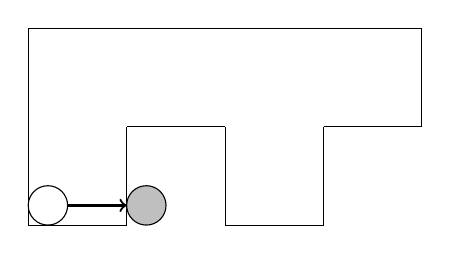
\begin{tikzpicture}
			\draw (0, 0)--(5, 0);
			\draw (5, 0)--(5, -1.25);
			\draw (5, -1.25)--(3.75, -1.25);
			\draw (3.75, -1.25)--(3.75, -2.5);
			\draw (3.75, -2.5)--(2.5, -2.5);
			\draw (2.5, -2.5)--(2.5, -1.25);
			\draw (2.5, -1.25)--(1.25, -1.25);
			\draw (1.25, -1.25)--(1.25, -2.5);
			\draw (1.25, -2.5)--(0, -2.5);
			\draw (0, -2.5)--(0,0);
				
			\draw (0.25, -2.25) circle (0.25);
			\draw[fill=gray!50] (1.5, -2.25) circle(0.25);
								
			\draw[->, thick] (0.5, -2.25) -- (1.25, -2.25);
			\end{tikzpicture}
		\end{center}
		\caption{Расположение второй фигуры способом <<сквозного прохода>>}
		\label{second_through}
	\end{figure}